
\documentclass[12pt]{amsart}
\usepackage{geometry} 
\geometry{a4paper} 

\title{N\'omina}
\author{}
\date{}
\usepackage{graphicx} % to include images
\usepackage[export]{adjustbox} %adjusting position
\usepackage{subcaption} %using subfigures


\begin{document}
	

\begin{titlepage}
	\begin{center}
	\huge{\bfseries{Manual de Usuario}}\\
	[0.1cm]
	\line(1,0){300}\\
	\textsc{\small{Emilio Cant\'on}}\
	\textsc{\small{Roberto Gervacio}}\
	\textsc{\small{Yann Le Lorier}}
	\begin{figure}
		
\includegraphics[width=\linewidth]{Tec.jpg}
		\label{fig:Tec}
	\end{figure}
	
	\end{center}

\end{titlepage}

\maketitle
\tableofcontents

\section{Introducci\'on}
{El programa que hemos escrito en \textit{Java} nos permite visualizar una ventana gr\'afica que, al iniciar una sesi\'on de administrador, habilita todos los botones del programa. Los botones son habilitados as\'i como los \textit{TextFields}.}

\section{La ventana gr\'afica}
\subsection{Iniciar Sesi\'on}
{Es necesario introducir un usuario y una contrase\~na v\'alidos para poder habilitar las funciones del programa. De lo contrario, no se pueden hacer registros o cambios en la n\'omina.(\textit{cf} figura ~\ref{fig:Login})}\\
{En la ventana para iniciar sesi\'on (figura ~\ref{fig:Login}) es necesario ingresar un usuario y contrase\~na v\'alidos, por el momento existe un solo usuario v\'alido. Por defecto, el \'unico usuario es \textit{rob} y su contrase\~na es \textit{123}.}

\subsection{Ventana de matr\'iculas y de nombres completos}
{Aqu\'i aparecen todas las n\'ominas de los empleados. En caso de querer visualizar la informaci\'on de un empleado en espec\'ifico, s\'olo se tiene que hacer click en el campo deseado, por lo que pasamos a la siguiente secci\'on.\textit{cf} figura ~\ref{fig:sueldo}.}

\subsection{Informaci\'on detallada}
{Aqu\'i es posible ver la infomaci\'on en detalle de una persona en espec\'ifico, as\'i como es posible realizar cambios.}\\
{Para realizar cambios, es necesario hacer click en el bot\'on de \textit{editar}. \textit{cf} figura ~\ref{fig:Info} }\\\\\\\\\\\\\\\\\\\\\\

\begin{figure}[h]
	\begin{subfigure}{0.5\textwidth}
	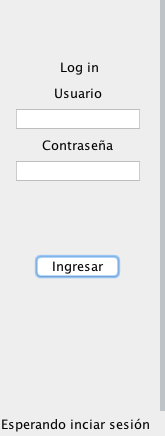
\includegraphics[width=20mm]{Login.jpg}
	\caption{Ventana de inicio de sesi\'on}
	\label{fig:Login}
	\end{subfigure}
	\begin{subfigure}{0.5\textwidth}
	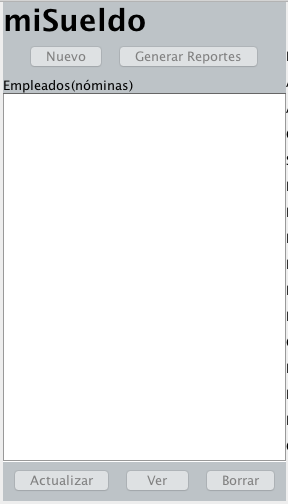
\includegraphics[width=20mm]{sueldo.png}
	\caption{Ventana de n\'ominas}
	\label{fig:sueldo}
	\end{subfigure}
	\begin{subfigure}{0.5\textwidth}
	\includegraphics[width=50mm]{info.jpg}
	\caption{Informaci\'on detallada}
	\label{fig:Info}
	\end{subfigure}
	\caption{La Ventana gr\'afica}
\end{figure}

\section{Recomendaciones}
\begin{itemize}
\item Ejecutar el programa en un Sistema operativo basado en Unix (Mac, Linux)
\item Es preferible meter el archivo miSueldo.jar en una carpeta en espec\'ifico, ya que el programa generar\'a otros archivos que pueden ser molestos
\item Tener un programa que abra los .csv
\item No modificar la base de datos manualmente
\end{itemize}


\section{Administraci\'on de Usuarios}
\subsection{Dar de alta a usuarios}
{Para dar de alta a usuarios, es necesario iniciar sesi\'on (figura ~\ref{fig:Login}), posteriormente, hacer click en el bot\'on \textit{Nuevo}, dentro de la ventana de n\'ominas (figura ~\ref{fig:sueldo}), despu\'es llenar todos los campos de los datos de la nueva persona en la ventana de datos personales (Figura ~\ref{fig:Info}), aqu\'i los datos requeridos:}
\begin{itemize}
\item Nombre : String (s\'olo letras)
\item Apellido Paterno : String (s\'olo letras)
\item Apellido Materno : String (s\'olo letras)
\item N\'omina : double
\item Cargo : String (s\'olo letras)
\item Sueldo : double
\item D\'ias trabajados : int (de 1 a 365)
\item Horas extra : int
\item Bonos : double
\item Otras asignaciones : double
\item IVA (16\%, se asigna autom\'aticamente, inmutable)
\item ISR (se asigna autom\'aticamente, inmutable)
\item Pr\'estamos : double
\item Otras deducciones : double
\end{itemize}

{En caso de agregar un nuevo empleado, Hacer click en el bot\'on \textit{Nuevo}, y llenar los datos correspondientes.}\\


{ Finalmente, hacer click en \textit{Guardar}. }

\subsection{Dar de baja a usuarios}
{Para dar de baja a usuarios, es necesario acceder a la ventana de N\'ominas (figura ~\ref{fig:sueldo}), despu\'es desplazarse hacia abajo hasta encontrar la n\'omina que se desea dar de baja. Dar un solo click en la n\'omina y despu\'es dar click en \textit{Borrar}.}

\subsection{Modificar datos de un empleado}
{Para modificar los datos de un empleado en espec\'ifico, se debe de seleccionar en la ventana de N\'ominas (figura ~\ref{fig:sueldo}), la que pertenece al empleado al que le deseamos hacer cambios.}\\
{Ahora desplazar el cursor hacia el bot\'on de \textit{Ver}. Aparecer\'a toda la informaci\'on del empleado en la ventana de la informaci\'on detallada (figura ~\ref{fig:Info}), Hacer click sobre el bot\'on de \textit{Editar}, y hacer los cambios necesarios. \textit{No olvidar de guardar los cambios.}}

\subsection{Nota}
{Si no encuentra al empleado deseado, haga click en el bot\'on \textit{Actualizar}, para ver todos las n\'ominas existentes en la base de datos.}\\
{Si desea sabes exactamente cu\'al es el formato de un \textit{TextField}, simplemente sobrevolar \'este \'ultimo, un peque\~no \'icono aparecer\'a al lado del cursor.}

\end{document}